\chapter{Trainingswissenschaftliche Grundlagen}
\label{sec:grundlagen:rad}
Vor der Erstellung eines Modells gilt es die Merkmale eines optimalen Trainingsverlaufs zu spezifizieren. Dabei gibt es allgemeingültige sowie sportartspezifische Prinzipien der Gestaltung einer Trainingseinheit sowie darin enthaltener Trainingsabschnitte.

\section{Trainingsziel}
Orientiert sich das Trainingsziel an einem Wettkampf, stellt sich immer die Frage nach der Wettkampfdisziplin. Sportarten umfassen unterschiedliche Disziplinen, die jeweils andere Leistungsprofile erfordern. Im Radsport gibt es ein weites Spektrum -- von weltbekannten Etappenrennen wie der Tour de France bis hin zu Bahnradrennen. Diese beiden Beispiele gehen jedoch über die Zielgruppe dieser Arbeit hinaus, denn die Teilnehmenden erhalten professionelle Trainingsbetreuung, wie im Profisport üblich. Im Amateursport sind dagegen folgende Wettkampfarten von größter Bedeutung.
\subsection{Eintagesrennen/Straßeneinzelrennen}
\label{eintagesrennen}
Das Eintagesrennen ist die älteste und verbreitetste Form der Straßenradrennen. Den ersten Platz erlangt die Person, die am schnellsten die Ziellinie erreicht.
Üblicherweise beträgt die zurückzulegende Strecke weniger als 250 km. Die Belastung ist eng an das Streckenprofil (flach, wellig oder bergig) gekoppelt. So ist auch die Energiebereitstellung breit gefächert. Das Training betrifft diverse Belastungsbereiche mit Fokus auf die Ausdauer.
Ein ähnliches Belastungsprofil gilt beim Zeitfahren. Hier starten die Fahrer:innen jedoch einzeln und die gefahrenen Zeiten werden im Anschluss verglichen. Auf die Gewichtung der Belastungsbereiche hat dies jedoch keinen Einfluss. 
\subsection{Rundstreckenrennen}
Diese Disziplin unterscheidet sich von Eintagesrennen in der Länge der Strecke und der Art der Wertung. Eine Runde ist mit 800 Metern bis 10 Kilometern relativ kurz. Ein Rennen besteht aus mehreren Runden. 
Das beeinflusst maßgeblich das Leistungsprofil. Durch die Kürze der Strecke verliert die Ausdauer etwas an Bedeutung. Kraft und Schnelligkeit hingegen sind in diesem Wettkampf relevanter. In die Wertung fließen nämlich zusätzliche Punkte für Sprints ein. Bei diesen handelt es sich um kurze Teilstrecken innerhalb eines Rennens. 

\subsection{Bergzeitfahrt}
Wie in \ref{eintagesrennen} aufgegriffen, differenziert sich das Zeitfahren durch die Messung der Zeiten in aufeinanderfolgender Reihenfolge. Für die Definition der Belastungsbereiche entscheidend ist hier aber das Streckenprofil. Gesondert betrachtet wird demnach das Fahren am Berg, sogenannte Bergzeitfahrten. Bei Strecken mit hohen Anstiegen konzentriert sich die Leistung auf hohe Intensitäten. In dieser Wettkampfdisziplin ist die Kraft von zentraler Bedeutung, um den Anstieg zu meistern.

\section{Trainingsprinzipien}
\subsection{Periodisierung}
Zweck eines Trainingsplans ist es, in einem definierten Zeitrahmen individuelle Einheiten einzuplanen, um das persönliche Trainingsziel zu erreichen. Daraus hergeleitete Teilziele dienen einer detaillierteren Struktur. Die Granularität kann sogar bis zu einer individuellen Ausrichtung der Woche reichen. Jedes Teilziel wird in einer Periode behandelt, die Einfluss auf den Inhalt der Trainingseinheiten hat. \cite{periodization} \par
Im Falle eines wettkampforientierten Trainingsjahres strebt man zum Wettkampf die maximale Leistungsfähigkeit an. Typischerweise setzt sich ein Trainingsjahr aus Vorbereitungsperiode, Aufbauperiode und Übergangsperiode zusammen. \cite[279]{Trainingswissenschaft}  \newline
Die Vorbereitungsperiode umfasst die Grundlagenausdauer und allgemeine Fitness. Im Radsport liegt diese im Allgemeinen in der Wintersaison. \newline
Innerhalb einer Aufbauperiode werden zunehmend die wettkampfspezifischen Fähigkeiten ausgebaut. Das Training wird auf die individuellen Anforderungen eines Wettkampfs abgestimmt. Dabei kann abhängig von Länge und Anzahl der Wettkampfperioden einfach oder mehrfach periodisiert werden. \newline
Auf den Wettkampf folgt die Übergangsperiode. Der Trainingsumfang ist hier gesenkt, um dem Körper Erholung zu ermöglichen.

\subsection{Zyklisierung}
Das Training gliedert sich in verschiedene Zyklen mit hierarchischem Aufbau. Sie geben dabei die Belastung und Regenerationsphasen im Trainingsplan vor. Übergeordnete Stufen wirken auf darunterliegende Zyklen ein, indem sie den Trainingsumfang, die Methoden und auch die Wahl der Belastungsbereiche beeinflussen. \cite[283]{Trainingswissenschaft}
Makrozyklen haben eine Dauer von drei bis fünf Monaten. Sie bestehen aus Mesozyklen, die eine Dauer von circa vier Wochen haben. Jede Woche wird dabei als Mikrozyklus bezeichnet. Darin werden die Trainingseinheiten geplant. Sogenannte strukturierte Trainingseinheiten definieren zusätzlich die enthaltenen Trainingsabschnitte. Maßgeblich für die Unterteilung einer Einheit ist dabei die Trainingsmethode. Eine Übersicht dieser folgt in \hyperref[grundlagen:methoden]{Kapitel \ref{grundlagen:methoden}}.

\subsection{Progressive Belastungssteigerung}
Die Gestaltung der Mesozyklen folgt direkt aus dem Prinzip der progressiven Belastung. Nach einem Trainingsreiz über der Reizschwelle reagiert der Körper mit Anpassungen. Die Leistung wird gesteigert, indem die Reizschwelle erhöht wird. Weitere Leistungssteigerungen durch Anpassungen des Körpers treten erst ein, wenn die veränderte Reizschwelle übertroffen wird. Die Belastung durch Trainingseinheiten erzielt eine optimale Leistungssteigerung, wenn sie progressiv gestaltet ist. Jedoch schädigt ein zu starker überschwelliger Reiz das System. Bei unterschwelligen Reizen führen die Trainingseinheiten nicht zur Steigerung der Leistung, da keine körperliche Anpassung stattfindet. \cite[58]{Seidenspinner2005} Progression kann dabei durch Steigerung der wöchentlichen Trainingstage, der Dauer der Einheiten oder der Trainingsintensität erreicht werden. Möglich ist auch die Verkürzung der Pausen.\newline 
Mesozyklen und Makrozyklen sind jeweils mit steigender Belastung geplant. Der Trainingsumfang dient hierbei als Richtwert. \cite[60-61]{Radsporttraining} Bei Mesozyklen wurde eine 3:1 Periodisierung vorgenommen. Dabei wird die ersten drei Wochen mit steigender Belastung trainiert. Im Anschluss folgt eine Regenerationswoche mit reduziertem Umfang.

\subsection{Regeneration}
Die Anpassung des Körpers an neue überschwellige Reize erfolgt nicht beim Training selbst, sondern in der Regenerationszeit. Um Übertraining zu verhindern, ist mindestens ein Regenerationstag in der Woche einzuplanen. \cite{EinfuerungTrainingswissenschaft}
Zur optimalen Leistungssteigerung werden sowohl Trainingseinheiten als auch Belastungspausen zwischen den Einheiten eingeplant. Die Länge der Regenerationspause ist dabei abhängig von Intensität und Dauer der vorangegangenen Leistung. Auch Alter, Geschlecht, Ernährung oder Tagesform spielen eine Rolle. Trotzdem verlieren einige Richtlinien nicht die Allgemeingültigkeit. Beispielsweise folgt nach Wettkämpfen immer eine Phase der Regeneration. Diese kann auch als aktive Regeneration gestaltet sein. Das sind Trainingseinheiten mit geringster Intensität.

\subsection{Superkompensationsmethode}
Die Superkompensation bezeichnet die gesteigerte Leistungsfähigkeit bei optimaler Zeitplanung der Regeneration nach einer Belastung. \cite[163]{Trainingswissenschaft} Dabei ist Übertraining, aber auch Unterforderung zu vermeiden, um eine bestmögliche Belastung zu erreichen. In der Erholungsphase gibt es einen Zeitpunkt, an dem erhöhte Leistungsbereitschaft besteht. Der Zeitpunkt ist abhängig von Intensität und Umfang der jeweiligen Einheit, aber auch von persönlichen Voraussetzungen wie Leistungsstand und Erholungsfähigkeit. \newline
Folgende Richtlinien ergeben sich für die Trainingsplanung \cite[44-46]{Radsporttraining}: Nur eine Trainingseinheit pro Tag wird bei mehrstündigen Ausdauerbelastungen eingeplant. Die Belastung sollte dabei im Block erfolgen -- circa drei bis fünf aufeinanderfolgende Tage bei Einheiten für die Grundlagenausdauer. Bei Einheiten mit hoher Intensität sind die Blöcke kürzer gestaltet. Im Anschluss an einen Belastungsblock folgt ein Regenerationstag. An Erholungstagen ist keine Trainingseinheit oder maximal eine Belastung im Regenerationsbereich erlaubt. Einheiten im Bereich des Krafttrainings werden bevorzugt nach einem Regenerationstag eingeplant. \cite[60]{Radsporttraining}

\section{Belastungsbereiche}
\label{grundlagen:sport:belastungsbereiche}
Die Aufbauperiode dient zur Vorbereitung auf einen Wettkampf. Im Radsport gibt es verschiedene Disziplinen (Straßenrennen, Zeitfahrten, Bergfahrten, uvm.) mit unterschiedlichem Belastungsprofil. Um die wettkampfspezifischen Anforderungen zu trainieren, werden die Belastungsbereiche des Radsports in deren Abhängigkeit gewichtet. Maßgeblich ist die Intensität der Belastung. Folgende Einteilung der Bereiche findet man in Lindners Radsporttraining. \cite[31-39]{Radsporttraining} Obwohl die Benennung nicht übereinstimmt, wurde in vergleichbarer Literatur \cite[27]{Ausdauertrainer} eine analoge Einteilung in sieben Stufen vorgenommen. 
\subsection{Kompensationsbereich KB}
Der Belastungsbereich mit niedrigster Intensität ist der Kompensationsbereich. Dieses Training belastet mit 60 Prozent der maximalen Herzfrequenz. Es wird zur aktiven Regeneration oder Kompensation eingesetzt. Üblicherweise folgt ein Kompensationstraining nach sehr intensiven Einheiten oder Wettkampfbelastungen. Beispiele für ein Kompensationstraining sind Ausfahrten oder Läufe mit geringer Intensität, Spaziergänge oder Mobilisationstrainings. \cite[31-32]{Radsporttraining}
Eine Regenerationsfahrt hat eine maximale Länge von zwei Stunden. Das alternative Lauftraining sollte 45 Minuten nicht übersteigen und ist nur außerhalb der Radsaison ratsam.
\subsection{Grundlagenausdauer GA}
Trainingseinheiten mit leichter Intensität werden für die Entwicklung der Grundlagenausdauer verwendet. Bei Steuerung über die maximale Herzfrequenz kann von einem Richtwert von 80 Prozent ausgegangen werden. Es wird ausschließlich der aerobe Energiestoffwechsel beansprucht. Für das Verbrennen von Kohlenhydraten und Fetten wird dann Sauerstoff verwendet. Die Grundlagenausdauer nimmt einen großen Teil des Trainingsplans ein, da es sich beim Radsport um einen Ausdauersport handelt. Oft wird sie als Dauerleistung trainiert. Für intensive Einheiten wird aber auch ein Trainingsabschnitt im Grundlagenausdauerbereich eingeplant. Vor der intensiven Belastung dient er dem Aufwärmen und abschließend dem Ausfahren.
\subsection{Entwicklungsbereich EB}
Im Entwicklungbereich wird die wettkampfspezifische Ausdauer im mittleren Intensitätsbereich trainiert. Zusätzlich zum Fettstoffwechsel bindet es auch den Kohlenhydratstoffwechsel ein. Es wird im aeroben-anaeroben Bereich trainiert, der sowohl Sauerstoff aber auch Milchsäuregärung zur Energiegewinnung verwendet. Oft wird es als Wiederholungsmethode oder Intervallmethode durchgeführt.
\subsection{Spitzenbereich SB}
Bei hohen Intensitäten, wie im Spitzenbereich, erfolgt die Energiegewinnung aus Kohlenhydraten nicht mithilfe des Sauerstoffs. Hier wird der anaerobe Stoffwechsel beansprucht.
Ziel ist es, die Schnelligkeit und Schnelligkeitsausdauer auf die Wettkampfbedingungen zu entwickeln. Überwiegend sind Trainingseinheiten mit der Intervallmethode strukturiert und unmittelbar vor Wettkämpfen platziert.
\subsection{Maximal- und Schnellkraftsbereich K1-K2}
Im aeroben Bereich befindet sich die Entwicklung der Maximal- und Schnellkraft. Besonders bei Strecken mit hoher Steigung und Bergfahrten gewinnt dieser Bereich an Bedeutung. Außerdem profitieren Starts und Sprints vom Training in diesem Bereich, denn die Maximal- und Schnellkraft ermöglicht es, hohe Übersetzungen auch mit hoher Tretfrequenz zu beherrschen. Häufig wird dafür die Wiederholungsmethode eingesetzt. 
\subsection{Kraftausdauer K3-K4-K5}
Auch hier ist das Trainingsziel eine hohe Tretfrequenz mit hoher Übersetzung zu fahren. Diese soll nun auch über längere Zeit gehalten werden. Die Energiebereitstellung ist im aerob-anaeroben Übergangsbereich. Bergfahrten mit Tempo- und Rhythmuswechsel sind eine mögliche Trainingseinheit für diesen Belastungsbereich. \par

Bringt man Belastungsbereiche und Wettkampfdisziplinen zusammen, wird die Verlagerung der Schwerpunkte in den einzelnen Disziplinen sichtbar. Wettkämpfe mit höherem Streckenumfang erfordern mehr ausdauerspezifisches Training, das von niedriger Intensität geprägt ist. Kürzere Strecken, wie bei Zeitfahrten, erfordern Schnelligkeit, die vor allem in den Sprints wesentlich ist. Bergfahrten hingegen sind geprägt von der hohen Intensität und priorisieren deshalb Belastungsbereiche im Kraftbereich. Diese Tendenzen werden in \hyperref[fig:wettkampfLeistungsbereiche]{Abbildung \ref{fig:wettkampfLeistungsbereiche}} dargestellt. Dennoch ist anzumerken, dass die Werte von spezifischen Wettkampfstrecken abstrahieren und keine exakten Werte bestimmt werden können. 
\begin{figure}[hb]
    \centering
        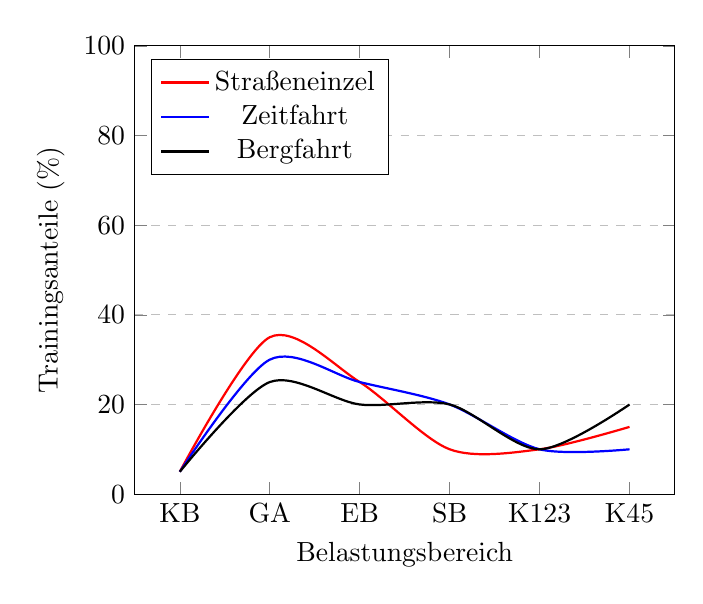
\begin{tikzpicture}
        \begin{axis}[
            xlabel={Belastungsbereich},
            ylabel={Trainingsanteile (\%)},
            xmin=-0.5, xmax=5.5,
            ymin=0, ymax=100,
            xticklabels={KB, GA, EB, SB, K123, K45},
            ytick={0,20,40,60,80,100},
            xtick={0, 1, 2, 3, 4, 5},
            legend pos=north west,
            ymajorgrids=true,
            grid style=dashed,
        ]
        \legend{Straßeneinzel, Zeitfahrt, Bergfahrt}
        
        \addplot[ % Straßeneinzel
            color=red,
            smooth,
            thick,
            ]
            coordinates {
            (0,5)(1,35)(2,25)(3, 10)(4, 10)(5,15)
            };
        \addplot[ % Zeitfahrt
            color=blue,
            thick,
            smooth
            ]
            coordinates {
            (0,5)(1,30)(2,25)(3,20)(4,10)(5,10)
            };
        \addplot[ % Bergfahrt
            color=black,
            thick,
            smooth
            ]
            coordinates {
            (0,05)(1,25)(2,20)(3,20)(4,10)(5,20)
            };
            
        \end{axis}
        \end{tikzpicture}
    \caption{Relevanz der Belastungsbereiche von Wettkampfdisziplinen nach \cite[30]{Radsporttraining}}
    \label{fig:wettkampfLeistungsbereiche}
\end{figure}
\section{Trainingsmethoden}
\label{grundlagen:methoden}
Um die Belastungsbereiche zu trainieren, kommen verschiedene Trainingsmethoden zur Gestaltung einer Trainingseinheit in Frage. Sie teilen eine Einheit auf unterschiedliche Weise in Trainingsabschnitte ein. Bezeichnet werden solche Einheiten auch als strukturierte Trainingseinheiten. Im Folgenden handelt es sich lediglich um eine Auswahl der möglichen Trainingsmethoden für Radsportler:innen in der Aufbauperiode. \cite[40-43]{Radsporttraining}
\subsection{Dauerleistungsmethode DL}
Bei der Dauerleistungsmethode wird die gesamte Trainingseinheit ohne Unterbrechung in einem Belastungsbereich ausgeführt. Bei höheren Intensitäten wird jedoch auch eine Aufwärmphase und Ausfahrzeit eingeplant. Die Grundlagenausdauer eignet sich hier, um Verletzungen zu unterbinden. Häufig findet diese Methode bei niedrigeren Intensitäten Verwendung. Ein Großteil der Vorbereitungsperiode priorisiert das Training des Grundlagenausdauerbereichs, der mit der Dauerleistungsmethode trainiert wird. \newline \hyperref[table:fahrtspiel]{Tabelle \ref{table:fahrtspiel}} führt die möglichen Trainingseinheiten dieser Methode auf. Anhand der Belastungsbereiche werden die möglichen Längen in einer Trainingseinheit festgelegt. Wie auch für die folgenden Methoden ist die Zeitspanne in Minuten angegeben und die Definition flexibel.
\newcolumntype{b}{>{\hsize=0.4\hsize}X}
\newcolumntype{s}{>{\hsize=0.1\hsize}X}
\begin{table}[h]
\centering  
\footnotesize
    \begin{tabularx}{\textwidth}{|b|ssssss|}
    \hline
    \rowcolor{ctcolorgraylight}
    \textbf{Einheit} & \textbf{KB} & \textbf{GA}& \textbf{EB}& \textbf{SB}& \textbf{K123}   &\textbf{K45} \\  \hline
    Kompensationsfahrt                  & 15-180 &         &             &        &        &           \\ \hline
    Extensive Fahrt                     &        & 30-300  &             &        &        &           \\ \hline
    Fettstoffwechselfahrt               &        & 60-300  &             &        &        &           \\ \hline
    Intensive Fahrt                     &        & 30-60 & 15-60       &        &        &           \\ \hline
    Extensive Kraftausdauer Fahrt       &        & 30-60   &             &        & 15-150 &           \\ \hline
    Einzelzeitfahrt                     &        & 30-60      &             & 15-60  &        &           \\ \hline
    \end{tabularx}
    \caption{Trainingseinheiten mit der Dauerleistungsmethode}
    \label{table:fahrtspiel}
\end{table}
\subsection{Fahrtspiel FS}
Das Fahrtspiel ist eine spezielle Art der Dauerleistungsmethode. Dabei gibt es keine Vorgaben hinsichtlich der Intensität und des Belastungsbereichs. Die Belastung erfolgt ohne Pause, kann aber mehrere Bereiche ansprechen und auch innerhalb einer Einheit flexibel in den Bereichen rotieren. Das freie Fahrtspiel unterliegt keiner Vorgabe bei der Gestaltung der Einheit. Das Training wird persönlich gesteuert oder kann durch die äußeren Gegebenheiten (bergiger Streckenverlauf) beeinflusst werden. Vorgaben über Anteile der Trainingsbereiche sind zeitlich flexibel eingebaut. Nicht jeder Belastungsbereich muss dabei abgedeckt werden. 

\begin{table}[h]
\centering  
\footnotesize
    \begin{tabularx}{\textwidth}{|b|ssssss|}
    \hline
    \rowcolor{ctcolorgraylight} 
    \textbf{Einheit}                     & \textbf{KB}     & \textbf{GA}      & \textbf{EB}          & \textbf{SB}     & \textbf{K123}   & \textbf{K45}       \\    \hline
    Extensives Fahrtspiel               &       & 15-240    & 15-240    &           &       &       \\\hline
    Intensives Fahrtspiel               &       & 15-300    & 15-300    & 15-300    &  0-180     & 0-180\\\hline
    \end{tabularx}
    \caption{Trainingseinheiten mit der Fahrtspielmethode}
    \label{table:fahrtspiel}
\end{table}

\subsection{Intervallmethode IV}
Intervalleinheiten alternieren Belastung und Erholungsphasen. Die Pausen reichen nicht für eine vollständige Erholung aus und können auch als aktive Pausen gestaltet werden. Bei aktiven Pausen wird das Training nicht vollständig unterbrochen, sondern mit geringer Aktivität weitergeführt. Serienpausen sind längere Pausen und gruppieren mehrere Belastungen. Besonders Einheiten mit hoher Intensität werden mithilfe der Intervallmethode trainiert. 
\begin{table}[h]
\centering
\footnotesize
    \begin{tabularx}{\textwidth}{|b|ssssss|}
    \hline
    \rowcolor{ctcolorgraylight} 
    \textbf{Einheit}                     & \textbf{KB}     & \textbf{GA}      & \textbf{EB}          & \textbf{SB}     & \textbf{K123}   & \textbf{K45}       \\    \hline
    Intensive Kraftausdauerfahrt &        & 30-90   &             &        &        & 15-120  \\\hline
    Schnelligkeitsausdauer               &        & 60-180  &             & 15-45  &        &           \\ \hline               
    \end{tabularx}
    \caption{Trainingseinheiten mit der Intervallmethode}
    \label{table:intervallmethode}
\end{table}

\subsection{Wiederholungsmethode WH}
Ähnlich wie in der Intervallmethode gibt es einen Wechsel zwischen Belastung und Erholung. Jedoch dienen die Pausen bei der Wiederholungsmethode der vollständigen Erholung. Anhand der Herzfrequenz kann kontrolliert werden, zu welchem Zeitpunkt die nächste Belastung startet. Auch hiermit werden tendenziell Trainingsbereiche mit hoher Intensität trainiert.
\begin{table}[h]
\centering
\footnotesize
    \begin{tabularx}{\textwidth}{|b|ssssss|}
    \hline
    \rowcolor{ctcolorgraylight} 
    \textbf{Einheit}                     & \textbf{KB}     & \textbf{GA}      & \textbf{EB}          & \textbf{SB}     & \textbf{K123}   & \textbf{K45}       \\    \hline
    Sprinttraining                       &        & 15-30   &             & 15-60  &        &       \\\hline           
    \end{tabularx}
        \caption{Trainingseinheiten mit der Wiederholungsmethode}
    \label{table:wiederholungsmethode}
\end{table}

Trägt man obige Ausprägungen einer Trainingsmethode zusammen, erhält man die Übersicht der Einheiten, die bei der Erstellung des Plans kombiniert werden können wie im Anhang unter \ref{anhang:trainingsarten}.